% vim: set tw=78 sts=2 sw=2 ts=8 aw et ai:
\documentclass[12pt]{article}

\usepackage[paper=a4paper, top=2cm, bottom=3cm, left=2.5cm, right=2.5cm]{geometry}

\usepackage{ucs}
\usepackage[utf8x]{inputenc}
\usepackage[english]{babel}
%\usepackage{hyperref}
\usepackage{underscore}	  % underscores need not be escaped
\usepackage{subfigure}
\usepackage{verbatim}
\usepackage{float}
\usepackage{booktabs}     % professional tables
\usepackage{parskip}
\usepackage{color}
\usepackage{combelow}
\usepackage{csquotes}
\usepackage{siunitx}

% Support for including graphics
\usepackage{graphicx}
\DeclareGraphicsExtensions{.pdf,.png,.jpg}

\newcommand{\todo}[1]{
	\colorbox{yellow}{
		\begin{minipage}{10cm}
			\textbf{TODO:}\\
			#1
		\end{minipage}
	}
}

\newcommand{\nextitem}{\par\hspace*{\labelsep}\textbullet\hspace*{\labelsep}}


\sisetup{
  group-four-digits = true,
  group-separator = {,}
}

\title{People Management in the IT industry}

\author{Alexandru-George BURGHELEA\\
Faculty of Automatic Control and Computers\\
University POLITEHNICA of Bucharest\\
Splaiul Independenței 313, Bucharest, Romania, 060042 \\
\emph{alexandru.burghelea@cti.pub.ro}}

\date{\today}

\begin{document}

\maketitle

\begin{abstract}
The scope of this paper is to examine different types of people management found in the software industries. It describes common ways to tackle people management alongside with common impediments observed in real life situations inside of corporations based in Bucharest. The study is viewed from the perspective of the relationships between people managers, direct reports and upper management.

\end{abstract}

\section{Introduction}
\label{sec:introduction}
Employees are the biggest asset a company can have and in the IT industry they can make the difference between the rise and fall of a business. 
The employees attitude and performance can easily make the difference between a \SI{1}[\$]{M} company and a \SI{10}[\$]{M} company.

One of the trickiest parts of a manager is people management, which means that he is in charge of motivating, training, courages and even defends the employees if the situation requires it. In the same time the manager is also in charge of firing, disciplining and evaluating his employees. Although this responsibilities usually seem to be at in opposition, the integration of both positive and negative aspects makes the difference between a successful and unsuccessful manager that is able to create a good and productive environment.

Although employees are considered human resources, they are not inventory and according to H. Ross Perot:
\begin{displayquote}
``People cannot be managed. Inventories can be managed, but people must be lead.''
\end{displayquote}
This already hints that the naming of \textit{people management} is a poor choice of words, but the responsibilities of a person in this position start to migrate from the management sphere into the leadership sphere.

\subsection{People Management Concept}
\label{sub-sec:pmconcept}

In big organizations, usually there is a hierarchy of management that helps keep the company running smoothly. Being a good manager is one of the toughest and sometimes the least acknowledged jobs. A manager has to both lead by example and also manage expectations. The management positions come in a lot of flavours varying from project management, branch management and ending with people management. 

Managers know that the critical difference between success and failure is made by the people. In the same time, surprisingly, there is little research demonstrating the link between people management and business performance. 

Although each company has it's own flavour of people management, it is very wide spread and accepted that a people manager is a person that manages one or more individuals and has the following attributions:
\begin{itemize}
\item hiring
\item creating job descriptions
\item creating and advising on career planes
\item performance evaluation
\item firing
\item receiving resignations
\end{itemize}

Overall the people manager job is a pragmatic and results oriented type of work where a person has to find the correct balance between company performance and employee satisfaction.

It usually has nothing to do with being a human resources person, but usually helps to have some HR knowledge (eg: legal notice period). 

Although a people manager usually focuses on the motivating and increasing the performance of the employees, they have to be aware that difficult situations (eg: firing) often arise and always keep in mind Donald Trumps quote:

\begin{displayquote}
``It's nothing personal. It's just business.''
\end{displayquote}

\subsection{Motivation}
\label{sub-sec:Motivation}

From June 2014 and until January 2015 I had the occasion to really get of my comfort zone because I was in a position of managing employees. The position I was in was very similar to \ref{sub-sec:techout}, having 4 direct reports outside of the technical team, but the difficult part came from the fact that that I also had a direct report from inside the project team, \ref{sub-sec:techin}. The trickiest part came from the fact that was also the team leader and the my direct report was also severely demotivated and did not want to do the same things in the project that she had been doing for the last months. On one side I had to make decisions that would favour the project but on the other hand I also had to factor into account her needs. It may seem like a simple solution to switch the owners of two modules, this was simply not possible because the other members were had more seniority and their skills were needed in other areas of the project, areas where the person in cause could not handle within the hard deadline of the team.

The motivation behind this report is to give an incentive over what a people manager role means and how to overcome some difficult situations that may arrive. My former manager once said about people manager that:
\begin{displayquote}
``They are the persons who wear two hats: a hat the represents the needs of the company and one that represents the desires of the employees.
\end{displayquote}
The most widespread difficulty that I observed among my people manager colleagues, especially the newly appointed ones was that most of us were not able to wear both the hats, dividing us into two camps: the people representatives (acting as a syndicate) and the company rulers (acting as a board of decision enforces).

\subsection{Objectives}
\label{sub-sec:objectives}


The objective of this paper is to propose solutions to tricky situations encountered as people manager. The second objective of this study is to elaborate a questionnaire based on my personal decision in coaching my direct reports in order to validate the correctness of my actions.

\section{Existing approaches}
\label{sec:existingapproaches}
\todo{Write Existing approaches chapters}
\newline

\subsection{Dedicated subdivision of the Human Resources department}
\label{sub-sec:hrdep}

\todo{Write about hr reps} \newline

\subsection{Technical person outside the project team}
\label{sub-sec:techout}

\todo{Write about tech member outside the project or outside the office} \newline

\subsection{Technical person from inside the team}
\label{sub-sec:techin}

\todo{Write about TL as PM} \newline



\section{Positioning inside the organizational structure of the company}
\label{sec:positioning}

\subsection{Management levels}
\label{sub-sec:levels}
\todo{Senior, Upper, Middle, Execution}
\newline

\subsection{Management abilities}
\todo{Management abilities, Paraschiv notes}

\subsection{Management relationships}
\label{sub-sec:relationships}
\todo{small descriptions}

\subsubsection{People Manager - Direct Report}
\label{sub-sub-sec:pmdr}
\todo{You with your people} \newline

\subsubsection{People Manager - Upper Management}
\label{sub-sub-sec:pmum}
\todo{You with your bosses} \newline



\section{Tools for people management}
\label{sec:tools}

\subsection{Performance Formula}
\label{sub-sec:formula}
\todo{perf = want and can} \newline

\subsection{PRAE Model}
\label{sub-sec:prae}


Each person has it's own personality and from a psychological point of view there are different indicator types. One of these indicators are the Myers-Brigs indicator \cite{myers} (based on the research of C. Jung) and offer 8 personality traits that result in 16 personality types. This traits are:
\begin{itemize}
\item extroversion(E) / introversion (I)
\item sensing (S) / intuition(N)
\item thinking (T) / feeling (F) 
\item judgement (J) / perception (P)
\end{itemize}
Each person has one of the two traits from each of the categories above, and the different combination result in 16 possible personalities. Their interpretations can be found at \cite{mbf}.

Although the Myers-Brigs indicator was intended to be used by people with no qualifications in psychology, in practice it has proven very difficult for managers to identify the correct traits of their employees without using extensive tests. A simpler model was developed in order to help managers in interacting with their employees based on their personality. 

\begin{figure}[h]
\centering
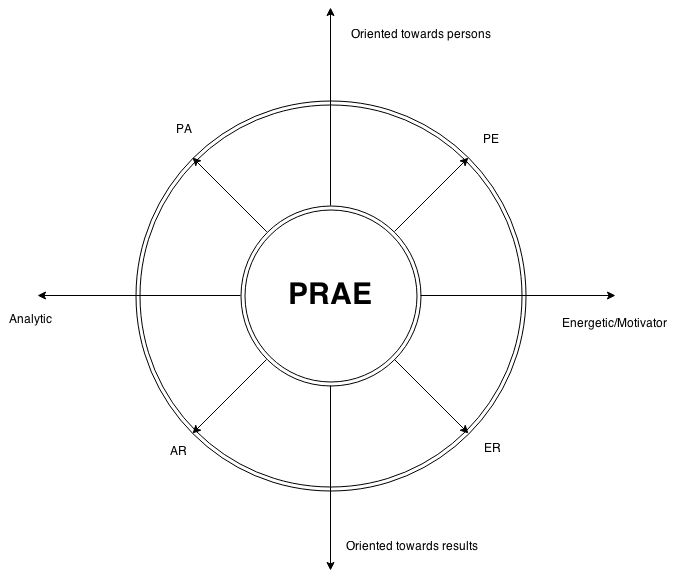
\includegraphics[width=0.8\textwidth]{img/prae.png}
\caption{PRAE personality model}
\label{fig:prae}
\end{figure}

The \textbf{PRAE} model is based on 4 traits, and as the name suggest the traits are:
\begin{itemize}
\item Person oriented
\item Result oriented
\item Analytical
\item Energetic(motivator)
\end{itemize}

Based on the PRAE model, each parson has a dominant trait that he uses in most situations and is usually the way that a person feels most comfortable to act as. A person also has a secondary trait that he usually uses in unusual/under-pressure situations. At the opposite end there is the adverse trait that hints the behaviour that a person is least comfortable to use.



In \ref{fig:prae} the vertical axis (P-R) is called \textit{Scope of action} and the horizontal axis (A-E) is called the \textit{Style of action}. As \ref{fig:prae} hints(although not impossible) the dominant and secondary traits are usually found on different axis. 

Although there are a lot of questionnaires to determine the PRAE model for each person, the dominant and secondary trait can be easily determined by the language that a person uses. In \ref{table:prae} can be found a description of the strong points, weak points and language indicator according to each PRAE trait.

\begin{table}[h]
  \centering
  \caption{Prae dreakdown detalis}
  \setlength\tabcolsep{3.8pt}
  \setlength\extrarowheight{1pt}
    \begin{tabular}{ | p{0.11\textwidth} | p{0.3\textwidth} | p{0.3\textwidth} | p{0.29\textwidth} |}
    \hline
    Trait & Strong points & Week Points & Language Indicators \\ \hline
    
    Person oriented 
     &
      \begin{itemize}
      \item he cares
      \item tactful
      \item motivating
      \item peacemaker, pacifist
      \item looks for cooperation and consensus
      \item tries to involve all the parties
      \end{itemize}
     & 
      \begin{itemize}
      \item easily offend
      \item very emotive
      \item listens to "what the others say"
      \item constantly looking for approval
      \item wishes to please everybody
      \item procrastination in making decisions
      \end{itemize}
     & 
      \begin{itemize}
      \item words like \textit{we, together}
      \item protective vocabulary
      \item do not get straight to the point
      \item spoiled behaviour
      \end{itemize}
     \\ \hline
    Results oriented
     &
      \begin{itemize}
       \item focuses on end result
       \item competitive
       \item honest and straight forward
       \item risk takers
       \item work well under pressure
      \end{itemize}
     &
      \begin{itemize}
       \item do not have patience with people
       \item sometimes sarcastic and insensible
       \item anti rules or processes
       \item individualists
       \item think in black or white
       \item become frustrated by persons who are afraid of risks
      \end{itemize}
     & 
     \begin{itemize}
      \item phrases like: I want
      \item Asks for facts and numbers
      \item Asks \textit {What's in it for me}
      \item Short time spent talking about \textit {how to do it}
     \end{itemize}
     \\ \hline
    Analytical
     &
      \begin{itemize}
       \item precise
       \item looks for proof and validation
       \item plans everything in a step by step way
       \item focused on facts and numbers
       \item sets high standards
      \end{itemize}
     &
      \begin{itemize}
       \item favours processes over results or relationships
       \item tendency to pessimism
       \item critic
       \item suffers from \textit{Paralysis by Analysis}
       \item can portrait intellectual arrogance.
      \end{itemize}
     &
      \begin{itemize}
       \item words like: must and depends
       \item asks for all the details
       \item gets irritated if interrupted
       \item gets frustrated when told how to do his work
      \end{itemize}
     \\ \hline
    Energetic 
     &
      \begin{itemize}
       \item enthusiast
       \item likes variety
       \item creates a friendly environment
       \item persuasive 
       \item spontaneous
       \item likes to have fun
       \item optimist
      \end{itemize}
     &
     \begin{itemize}
      \item impulsive
      \item thinks out loud
      \item disorganized, superficial
      \item easily bored
      \item skips analysis
      \item looks for attention and recognition
     \end{itemize}
     & 
      \begin{itemize}
       \item excessive use of words hinting his person: Me, I 
       \item makes himself the center of attention
       \item reacts positively to phrases like: You can, You will
      \end{itemize}
     \\ \hline
    \end{tabular}
    \label{table:prae}
\end{table}
\FloatBarrier

In the IT industry I observed that in 50\% of cases the combination between dominant and secondary trait is formed from \textit{Analytical} and \textit{Results}. This kind of persons are real assets to a company that is already established and focusses more on quality and not on delivering new features using short deadlines. For continuing to add new value to a product a person that has a mix made from \textit{Results} and \textit{Energetic} person is needed. The biggest drawback I observed for this mix is that this kind of person easily looses it's focus if something new needs to be implement, thus starting to work on new things without analysing all the possible use-cases and delivering software that works only on positive scenarios.
\subsection{RACI Matrix}
\label{sub-sec:raci}
\todo{RACI} \newline

\subsection{FAC Model}
\label{sub-sec:fac}
\todo{FAC feedback} \newline

\section{Impediments in people management}
\label{sec:impediments}
\subsection{Setting incorrect development objectives}
\label{subsec:devobjectives}
\todo{non-SMART, non-PEPSI}
\newline

\subsection{Interpersonal Conflicts}
\label{subsec:conflicts}
\todo{Conflicts between PM and DR}
\newline

\subsection{Incorrect delivery and interpretation of feed-back}
\label{subsec:incorrectfeedback}
\todo{How to correctly deliver and interpret feed-back}
\newline

\subsection{Incoherence between people managers}
\label{subsec:incoherence}
\todo{What happens when people managers do not send the same message}
\newline



\section{People management in other fields}
\label{sec:otherfields}
Although not really widely used in an official manner, people management techniques can be seen in other fields.
\subsection{Military Field}
\label{subsec:military}
The army has to always keep the morale of their troops high (especially in war theatres). In order to obtain this, they will sometimes set up shows and arrange leaves for the soldiers to visit their families. When the commanders prove that they care more about the troops instead of their own person there has been seen to improve the morale. One situation of this is described by Sinek in \cite{safe} about Cpt. William Swenson. Cpt Swenson preferred to rush in and retrieve his injured soldiers, putting himself in the middle of cross fire. In this way he proved that his troops were more important than his own safety. As a result, the soldiers that were returning fire were even more motivated to eliminate the threat fast.

\subsection{Legal Field}
\label{subsec:legal}
In law firms coaching is very visible, while a new employee usually start as an junior associate he is responsible with digging through the paperwork and find the proof that helps his case (or even loopholes in the laws). After a couple of years, after he has gather experience in the courtroom alongside senior colleagues he is promoted to an associate level. In this situation trust is given to him, because he is allowed to be a led attorney for some cases. His senior colleagues will monitor his performance and provide feedback. When a senior position is open, the most promising associate is promoted and know he becomes in charge of training junior associates.


\section{Conclusion and Future Work}
\label{sec:conclusion}
% vim: set tw=78 sts=2 sw=2 ts=8 aw et ai:
Based on the details above, a leader has to evaluate his decisions and ask himself what can he do to correct the situation. While a leader coordinates a team he has to take into account what is the time frame that he has until project delivery is needed. This is important in order to decide if a \textit{Leader-Follower} or \textit{Leader-Leader} approach is more suited. It's the leaders responsibility to create slack time so that he creates a good environment for the team to learn new skills and he also has to take into account that his success is a direct result of the teams efforts. While leading a team it is important to delegate part of the tasks so that each team member has the occasion to get a clear picture of what leadership means. In the same time it is important to create personal relationships with the members so that they can be motivated accordingly and also to avoid a high turn-over rate.

\subsection{Questions a leaders has to answer in order to validate his leadership approach}
In team coordination there is no fool proof recipe for success, in the same time a leader can evaluate his actions on a high level. Every team leader should be able to know how to answer the following questions:

\begin{enumerate}
\item \textbf{What kind of leader do I want to be? (Technical decision maker or Team leader/Coach)} The leader has to know what are his expectations from himself.
\item \textbf{What is the lifespan of the team?} If a leader will coordinate a team for a single and short-lived project it may not be feasible to create slack time.
\item \textbf{Do I know each member in person and how he thinks? If not how do I obtain this information?} Without really knowing each team member a leader will not know how to correctly motivate each individual.
\item \textbf{What phase is the team in?} Creating a self organizing team can not be achieved by burning phases. A team has to go through day-by-day phase and then a learning phase in order to truly become self-organizing.
\item \textbf{If I suddenly leave the team, will it do better or worse?} If the answer is worse and the goal is to have a self organizing team then it means that the leadership is either incorrect or incomplete
\item \textbf{How can I teach my team to not fear failure} Leadership is often done by example. If the leader proves that he is able to risk even if the repercussions could be devastating.
\item \textbf{What tasks can I delegate and to whom} Not any task on the leaders plate can be delegated. A leader must correctly identify the person that is both willing and wishing to do his tasks?
\item \textbf{Does my team have enough time to learn?} Without developing the skills of a team progress is absent. Without progress de-motivation sets in.
\item \textbf{What would you and your team like to accomplish?} The project is not the answer to this question. To ensure the delivery on time, the team has to have a common goal.
\item \textbf{Are you unintentionally solving the teams problems instead of teaching them how to do it?} Coaching is the most important part of leadership. If a leader solves the problems of the team without teaching them how to solve them themselves he is not a leader, he is a commander.
\end{enumerate}

It is important to observe that there is no question about how the leader is seen by the team. It is important for a leader to be trusted, but it is not important to be liked.

\subsection{Future work}

For future development this paper will be enhanced by a study about team coordination and successful proven techniques in the Romanian industry. The study will be conducted by direct interviews and questionnaires with both team leaders and team members to observe the rate of success of common decisions.Also a comparison between the teams expectations and management expectations will be.

In order to develop a more in-depth vision about team leadership, the position will be studied form a point of view where a team leader has to set expectations from his team while coordinating with the senior management in order to ensure company success. In the same time it is important to understand what are the expectations that a team members have from a team leader and what makes a difference between a good leader and a bad leader. It will also be studied what if a good leader is equal to a successful leader.

Team leadership is in general a hard task to do and usually the results are not always obvious. In order to create a self organizing team a leader has to continuously improve his management skills along side his technical skills. Decisions should be made based on both previous experience and also on team input. There is no guaranteed method for success and that is why there is always room for improvement. 

\section*{Acknowledgment}
\label{sec:acknowledgment}
The author would like to thank R\u{a}zvan Deaconescu for his support on elaborating this report. Also special thanks go to Adrian Zaiu, Phillip Luppens and Roxana P\u{a}duraru for showing me different ways to lead and motivate teams.

\bibliographystyle{abbrv}
\bibliography{people-management}

\end{document}
